\documentclass[11pt,a4paper]{article}

\usepackage[utf8]{inputenc}
\usepackage[T1]{fontenc}
\usepackage[margin=1in]{geometry}
\usepackage{hyperref}
\usepackage{xcolor}
\usepackage{listings}
\usepackage{longtable}
\usepackage{booktabs}
\usepackage{enumitem}
\usepackage{tikz}
\usetikzlibrary{arrows.meta, positioning, shapes.geometric, calc}
\usepackage{fancyhdr}
\usepackage{titlesec}

\definecolor{codebg}{RGB}{245,245,245}
\definecolor{accent}{RGB}{79,124,255}
\definecolor{accentdk}{RGB}{58,95,208}
\definecolor{danger}{RGB}{180,35,24}
\definecolor{dangerbg}{RGB}{252,232,232}
\definecolor{codekw}{RGB}{0,0,150}
\definecolor{codestr}{RGB}{140,70,20}
\definecolor{codecomment}{RGB}{100,120,100}
\definecolor{softgrey}{RGB}{150,150,150}

\hypersetup{colorlinks=true, linkcolor=accentdk, urlcolor=accentdk, citecolor=accentdk}

\lstdefinelanguage{jsonc}{
  morestring=[b]",
  morecomment=[l]{//},
  sensitive=true
}
\lstset{
  backgroundcolor=\color{codebg},
  basicstyle=\ttfamily\footnotesize,
  keywordstyle=\color{codekw}\bfseries,
  stringstyle=\color{codestr},
  commentstyle=\color{codecomment}\itshape,
  breaklines=true,
  frame=single,
  rulecolor=\color{gray!40},
  showstringspaces=false,
  columns=fullflexible,
  xleftmargin=8pt,
  xrightmargin=4pt
}

\pagestyle{fancy}
\fancyhf{}
\lhead{\small Parallel Multi-Agent Medical Intake}
\rhead{\small OpenPoke Implementation}
\cfoot{\thepage}

\titleformat{\section}{\Large\bfseries\color{accentdk}}{\thesection}{0.7em}{}
\titleformat{\subsection}{\large\bfseries}{\thesubsection}{0.6em}{}

\title{\textbf{Parallel Multi-Agent Medical Intake on OpenPoke}\\[4pt]
\large Implementation Document — Optimized Concurrent Agent Design}
\author{Build Trial — Voice AI Agent for Medical Office Intake \& Scheduling}
\date{\today}

\begin{document}

\maketitle
\thispagestyle{fancy}

\begin{abstract}
\noindent Detailed implementation for the handwritten design: a caller connects, a \textbf{voice agent} gathers
information into a shared file, a \textbf{medical agent} screens for a 911 emergency versus continuing intake,
and---if non-emergency---a \textbf{calendar agent} checks availability and books while a \textbf{gmail agent}
sends confirmation. The focus is the \emph{most optimized methodology for running these agents in parallel and
coordinating them together}, built on OpenPoke's existing asynchronous orchestration.
\end{abstract}

\tableofcontents
\newpage

% ==============================================================
\section{What This Reintroduces (Reconciliation)}

The handwritten note brings back \textbf{Gmail + Google Calendar via the OpenPoke (Composio) platform}. That is
compatible with the earlier constraints (reuse existing infrastructure, minimal new code, no new JavaScript,
Python, OpenRouter):

\begin{itemize}[leftmargin=*]
  \item \textbf{Gmail} already exists in OpenPoke (\texttt{tools/gmail.py} + \texttt{services/gmail/},
  Composio-backed). Reused as-is.
  \item \textbf{Google Calendar} is the one real addition: a new \texttt{tools/calendar.py} +
  \texttt{services/calendar/} that \emph{mirror the Gmail modules exactly} (same Composio client pattern).
  One new module, no new framework, no JavaScript.
  \item \textbf{Triage / medical reasoning} stays on \textbf{OpenRouter / Anthropic} via the existing client.
  No Gemini, GPT-direct, or database.
  \item \textbf{Patient information} is written to a \textbf{file} (as drawn), using OpenPoke's existing
  fcntl-locked JSON pattern.
  \item Every tool can fall back to a \textbf{mock} for the demo (the brief allows mocked tools) if Composio
  Calendar setup is a blocker---the concurrency design is identical either way.
\end{itemize}

% ==============================================================
\section{Agent Roster (Persistent, Specialized)}

Five long-lived roles. Keeping them \textbf{persistent and few} (not spawned per caller) is the first
optimization: it keeps the interaction agent's roster tiny and directly answers the brief's
``execution-agent overload'' discussion point.

\begin{center}
\begin{longtable}{@{}p{2.5cm}p{2.7cm}p{4.0cm}p{3.1cm}@{}}
\toprule
\textbf{Agent} & \textbf{OpenPoke basis} & \textbf{Responsibility} & \textbf{Session-file I/O} \\
\midrule
\endhead
\textbf{Interaction / Voice} & Interaction Agent (unchanged core) & Talks to caller, one question at a time, orchestrates, synthesizes & writes intake fields \\
\textbf{Medical / Triage} & Execution Agent + new \texttt{triage} task & Scans info, 911 vs.\ continue, assigns urgency & reads symptoms $\rightarrow$ writes \texttt{triage} \\
\textbf{Calendar} & Execution Agent + new \texttt{calendar} tools & Reads schedule, finds free slots, books event & reads \texttt{urgency} $\rightarrow$ writes \texttt{availability}, \texttt{booking} \\
\textbf{Gmail} & Execution Agent + existing \texttt{gmail} tools & Pulls prior context; sends confirmation & reads \texttt{booking} $\rightarrow$ writes \texttt{confirmation} \\
\textbf{Intake Record} & a \emph{tool}, not an agent & Atomic read/write of the session file & the file itself \\
\bottomrule
\end{longtable}
\end{center}

\noindent ``Intake Record'' is a tool rather than an agent on purpose---persisting a field should not cost an
LLM call.

% ==============================================================
\section{Coordination: A Shared Session-File ``Blackboard''}

This is how the agents work \textbf{together} while running in \textbf{parallel}. The note says
``stored in a file to save the info''; formalize that file as the single source of truth all agents read and
write, using the exact \texttt{fcntl.LOCK\_EX} pattern OpenPoke already uses for \texttt{roster.json}.

\textbf{Path:} \texttt{server/data/sessions/<call\_id>.json}

\begin{lstlisting}[language=jsonc]
{
  "call_id": "c_8f3a",
  "status": "intake",              // intake | emergency | scheduling | booked | handoff
  "caller":  { "name": null, "dob": null, "callback": null, "is_new": null },
  "intake":  { "symptoms": [], "insurance": null, "notes": null, "updated_at": null },
  "triage":  { "level": null, "urgency": null, "confidence": null, "rationale": null },
  "context": { "prior_visits": [], "existing_events": [] },
  "availability": [],              // [{slot_id, provider, start, end}]
  "booking": { "slot_id": null, "event_id": null, "confirmation_id": null },
  "confirmation": { "email_status": null, "message_id": null }
}
\end{lstlisting}

Why a blackboard beats passing data through prompts:

\begin{itemize}[leftmargin=*]
  \item \textbf{Decouples the agents} --- the calendar agent does not need the gmail agent in its prompt; it
  reads \texttt{booking} and writes \texttt{availability}. Parallel agents never block on each other's text.
  \item \textbf{Concurrency-safe} --- fcntl locking (already proven in \texttt{roster.json}) serializes writes;
  reads are cheap.
  \item \textbf{Crash / resume friendly} --- the file is durable state; any agent can be re-fired with full context.
  \item \textbf{Auditable} --- matches the brief's ``confirm critical details'' and yields a clean demo record.
\end{itemize}

\noindent Add a small \texttt{services/session/store.py} (copy \texttt{roster.py}'s lock logic) exposing
\texttt{read\_session(call\_id)} and \texttt{patch\_session(call\_id, partial)}.

% ==============================================================
\section{How OpenPoke Already Runs Agents in Parallel}

You are \textbf{not} writing an orchestrator---OpenPoke's is already asynchronous. The mechanics (verified in
the repository):

\begin{enumerate}[leftmargin=*]
  \item In \textbf{one} interaction-agent turn, the model can emit \textbf{multiple}
  \texttt{send\_message\_to\_agent} calls.
  \item Each call runs \texttt{roster.add\_agent(...)} then \texttt{loop.create\_task(\_execute\_async())} ---
  \textbf{non-blocking}. $N$ calls $\Rightarrow$ $N$ concurrent \texttt{asyncio} tasks.
  (\texttt{interaction\_agent/tools.py})
  \item \texttt{ExecutionBatchManager} registers each task as \textbf{pending} in one batch; each runs its own
  \texttt{ExecutionAgentRuntime.execute()} tool-loop ($\le 8$ iterations, 90\,s timeout).
  (\texttt{batch\_manager.py})
  \item When the batch \textbf{drains} (\texttt{pending == 0}), the manager formats a combined
  \texttt{"[SUCCESS] <agent>: <response>"} payload and calls the interaction agent's
  \texttt{handle\_agent\_message}---the \textbf{fan-in / synthesis} step.
  \item The interaction agent then replies to the caller and may dispatch the \textbf{next} batch.
\end{enumerate}

\begin{quote}
\textbf{Design rule:} put \emph{independent} work in the \emph{same} interaction turn (true parallelism); put
\emph{dependent} work in the \emph{next} turn (after the batch returns). The whole optimization problem is
deciding what is independent.
\end{quote}

% ==============================================================
\section{The Dependency Graph (Parallel vs.\ Sequential)}

\definecolor{softgrey}{RGB}{150,150,150}
\begin{center}
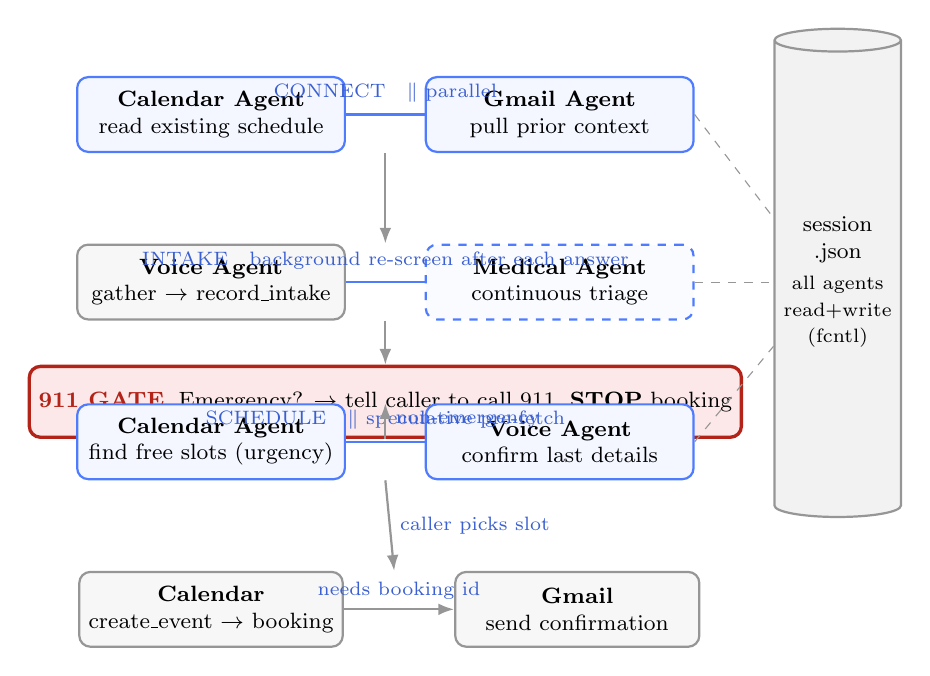
\begin{tikzpicture}[
  font=\footnotesize,
  pbox/.style={rectangle, rounded corners, draw=accent, thick, fill=accent!6,
               align=center, minimum width=3.4cm, minimum height=0.95cm},
  nbox/.style={rectangle, rounded corners, draw=softgrey, thick, fill=black!3,
               align=center, minimum width=3.4cm, minimum height=0.95cm},
  bgb/.style={rectangle, rounded corners, draw=accent, thick, dashed, fill=accent!3,
              align=center, minimum width=3.4cm, minimum height=0.95cm},
  stop/.style={rectangle, rounded corners, draw=danger, very thick, fill=dangerbg,
               align=center, minimum width=8.2cm, minimum height=0.9cm},
  fl/.style={-{Latex[length=2mm]}, thick, softgrey},
  pl/.style={-, thick, accent},
  lbl/.style={accentdk, font=\scriptsize}
]

% Phase 1 connect
\node[pbox] (cal1) {\textbf{Calendar Agent}\\read existing schedule};
\node[pbox, right=1.0cm of cal1] (gm1) {\textbf{Gmail Agent}\\pull prior context};
\draw[pl] (cal1) -- (gm1);
\node[lbl, above=1pt of $(cal1)!0.5!(gm1)$] {CONNECT \; $\parallel$ parallel};

% Phase 2 intake
\node[nbox, below=1.15cm of cal1] (voice1) {\textbf{Voice Agent}\\gather $\rightarrow$ record\_intake};
\node[bgb, right=1.0cm of voice1] (med) {\textbf{Medical Agent}\\continuous triage};
\draw[pl] (voice1) -- (med);
\node[lbl, above=1pt of $(voice1)!0.5!(med)$] {INTAKE \; background re-screen after each answer};
\draw[fl] ($(cal1.south)!0.5!(gm1.south)$) -- ($(voice1.north)!0.5!(med.north)$);

% barrier
\node[stop, below=1.05cm of $(voice1)!0.5!(med)$] (bar)
  {\textbf{\textcolor{danger}{911 GATE}}\; Emergency? $\rightarrow$ tell caller to call 911, \textbf{STOP} booking};
\draw[fl] ($(voice1.south)!0.5!(med.south)$) -- (bar.north);

% Phase 4 schedule
\node[pbox, below=1.05cm of voice1] (cal2) {\textbf{Calendar Agent}\\find free slots (urgency)};
\node[pbox, right=1.0cm of cal2] (voice2) {\textbf{Voice Agent}\\confirm last details};
\draw[pl] (cal2) -- (voice2);
\node[lbl, above=1pt of $(cal2)!0.5!(voice2)$] {SCHEDULE \; $\parallel$ speculative pre-fetch};
\draw[fl] (bar.south) -- node[lbl,right] {non-emergency} ($(cal2.north)!0.5!(voice2.north)$);

% Phase 5 book -> confirm
\node[nbox, below=1.15cm of cal2, minimum width=3.1cm] (book) {\textbf{Calendar}\\create\_event $\rightarrow$ booking};
\node[nbox, right=1.4cm of book, minimum width=3.1cm] (conf) {\textbf{Gmail}\\send confirmation};
\draw[fl] (book) -- node[lbl,above] {needs booking id} (conf);
\draw[fl] ($(cal2.south)!0.5!(voice2.south)$) -- node[lbl,right] {caller picks slot} ($(book.north)!0.5!(conf.north)$);

% blackboard
\node[cylinder, shape border rotate=90, aspect=0.18, draw=softgrey, thick, fill=black!5,
      minimum height=6.2cm, minimum width=1.6cm, align=center, right=1.0cm of med]
      (bb) {session\\.json\\[2pt]\scriptsize all agents\\\scriptsize read+write\\\scriptsize (fcntl)};
\draw[dashed, softgrey] (gm1.east) -- (bb.north west);
\draw[dashed, softgrey] (med.east) -- (bb.west);
\draw[dashed, softgrey] (voice2.east) -- (bb.south west);

\end{tikzpicture}
\end{center}

\noindent Parallel edges: the \textbf{connect reads}, and \textbf{free-slot lookup} $\parallel$ \textbf{final
questions}. Everything crossing the 911 barrier is sequenced. Booking\,$\rightarrow$\,confirmation is sequential
(confirmation needs the booking id) but each is one fast tool call.

% ==============================================================
\section{Phase-by-Phase Execution (Optimized)}

\subsection{Phase 1 --- Connect (parallel fan-out)}
On call start the interaction agent dispatches \textbf{two agents in one turn}: ask the Calendar Agent to read
today/tomorrow's schedule \emph{and} the Gmail Agent to pull prior caller context. They run concurrently;
results land in \texttt{context.existing\_events} / \texttt{context.prior\_visits}. Meanwhile the voice agent
greets the caller---so context pre-warms \emph{for free} during the greeting (latency hidden).

\subsection{Phase 2 --- Intake with continuous background triage (key optimization)}
Human conversation is inherently sequential, so do not fight it---\textbf{overlap triage with it}. Model the
Medical Agent like OpenPoke's \textbf{email watcher}: a background role that re-evaluates the session file
after every substantive answer rather than a single pass at the end.

\begin{itemize}[leftmargin=*]
  \item Voice agent: ask one question $\rightarrow$ \texttt{record\_intake} $\rightarrow$ continue.
  \item After each write, fire the Medical Agent \textbf{non-blockingly} with the current file. It returns
  \texttt{\{level, urgency, confidence, rationale\}}.
  \item Benefit: an emergency (``crushing chest pain'') is caught \textbf{mid-intake}, not after six
  questions---better safety \emph{and} lower latency. This is the single biggest win, and it is pure parallelism.
  \item Guard against noise: surface triage to the caller only when \texttt{level == emergency} or when intake
  is complete; otherwise it silently updates the file (reuse the existing \texttt{wait} discipline).
\end{itemize}

\subsection{Phase 3 --- 911 barrier (synchronization point)}
If any triage pass returns \texttt{emergency}: the interaction agent speaks the 911 instruction, sets
\texttt{status = "emergency"}, and a \textbf{guard in \texttt{calendar\_create\_event} refuses} while status is
emergency (defense in depth: prompt rule + code gate). No booking agent is dispatched.

\subsection{Phase 4 --- Schedule (parallel where possible)}
Non-emergency: once \texttt{triage.urgency} is set, dispatch the Calendar Agent's
\texttt{find\_free\_slots(urgency)} \textbf{in the same turn} as the voice agent's final confirmation questions
(insurance, callback number). Slots are ready by the time the caller finishes confirming---\textbf{speculative
pre-fetch}.

\subsection{Phase 5 --- Book $\rightarrow$ confirm (sequential, minimal)}
Caller picks a slot $\rightarrow$ Calendar Agent \texttt{create\_event} writes \texttt{booking} $\rightarrow$
interaction agent dispatches the Gmail Agent to send confirmation (reads \texttt{booking}) $\rightarrow$ voice
agent reads back the summary. Optionally schedule a \textbf{callback reminder} with the existing \textbf{Triggers}
system (free reuse).

% ==============================================================
\section{Optimizations Summary (for the README trade-offs)}

\begin{enumerate}[leftmargin=*]
  \item \textbf{Fan-out independent reads} at connect (calendar $\parallel$ gmail), hidden behind the greeting.
  \item \textbf{Continuous background triage} (watcher pattern) $\rightarrow$ early 911 detection, no
  end-of-call stall.
  \item \textbf{Shared fcntl-locked session file} $\rightarrow$ lock-free-feeling coordination; agents never
  block on each other.
  \item \textbf{Speculative slot pre-fetch} overlapping final questions $\rightarrow$ booking feels instant.
  \item \textbf{Persistent, few agents} (one per role) $\rightarrow$ tiny roster, no overload, context retained.
  \item \textbf{Tasks over tool-walls} $\rightarrow$ expose one \texttt{triage\_screen} task, not four endpoints.
  \item \textbf{Cheaper model on the hot path} $\rightarrow$ point \texttt{triage} at a smaller Anthropic id in
  \texttt{config.py}; keep Sonnet for the voice agent's language quality.
  \item \textbf{Defense-in-depth 911 gate} $\rightarrow$ prompt rule \emph{and} a code guard in the booking tool.
  \item \textbf{Idempotent booking} $\rightarrow$ key the event on \texttt{call\_id + slot\_id} so a retry never
  double-books.
\end{enumerate}

% ==============================================================
\section{Google Calendar Integration (the one new module)}

Mirror the Gmail modules 1:1 (Composio-backed, same \texttt{get\_active\_*\_user\_id} + \texttt{\_execute}
pattern):

\begin{itemize}[leftmargin=*]
  \item \texttt{server/services/calendar/client.py} --- copy \texttt{services/gmail/client.py}; expose
  \texttt{execute\_calendar\_tool} and \texttt{get\_active\_calendar\_user\_id}.
  \item \texttt{server/agents/execution\_agent/tools/calendar.py} --- copy \texttt{tools/gmail.py}; wrap these
  Composio Google Calendar actions (confirm exact slugs in your Composio dashboard, they can change):
  \begin{itemize}
    \item read schedule $\rightarrow$ \texttt{GOOGLECALENDAR\_FIND\_EVENT}
    \item availability $\rightarrow$ \texttt{GOOGLECALENDAR\_FIND\_FREE\_SLOTS} (or a free/busy query)
    \item booking $\rightarrow$ \texttt{GOOGLECALENDAR\_CREATE\_EVENT}
  \end{itemize}
  \item Register in \texttt{tools/registry.py} next to \texttt{gmail}.
  \item Add \texttt{COMPOSIO\_CALENDAR\_AUTH\_CONFIG\_ID} to \texttt{.env} / \texttt{config.py} (mirror the Gmail
  auth-config setting).
  \item Auth: add a Calendar OAuth connect action mirroring the Gmail settings flow (backend route only---reuse
  the existing settings UI, \textbf{no new JavaScript}).
\end{itemize}

\noindent \texttt{triage\_screen} is a \textbf{task} (new \texttt{tasks/clinic/}), not a Composio tool---it calls
OpenRouter/Anthropic through the existing client, exactly like the \texttt{search\_email} task calls the model
internally.

% ==============================================================
\section{Interaction-Agent Prompt Rules That Drive the Parallelism}

Add to \texttt{interaction\_agent/system\_prompt.md} (the model decides the batching, so the prompt must teach
it):

\begin{itemize}[leftmargin=*]
  \item ``At call start, in a \textbf{single} message, ask the Calendar Agent to read today's schedule
  \textbf{and} the Gmail Agent to pull prior context. Do not wait---greet the caller meanwhile.''
  \item ``After each caller answer, silently update the record and ask the Medical Agent to re-screen. Only
  interrupt the caller if it returns an emergency.''
  \item ``On emergency: tell the caller to call 911 immediately and do not book anything.''
  \item ``When urgency is set, ask the Calendar Agent for free slots \textbf{in the same message} you ask the
  caller your last confirmation question.''
  \item ``Only after the caller picks a slot, book it; only after booking succeeds, send the confirmation email.''
  \item ``Prefer one existing agent per role; never create a second Calendar/Gmail/Medical agent.''
  \item Keep the brief's guardrail: ``never diagnose, prescribe, or claim clinical certainty.''
\end{itemize}

\noindent Execution-agent prompts stay pure task machines (no personality)---the interaction agent owns voice/UX.

% ==============================================================
\section{Scope Tiers}

\textbf{MVP (works end-to-end, demoable):} session-file store; voice intake (existing chat UI, text);
continuous triage task + 911 gate; urgency; Calendar Agent with \textbf{mock} slots+booking; Gmail confirmation
(real, since Gmail already works); three scenarios; README.

\textbf{Full integration (if time):} real Composio Google Calendar (find/free/create); connect-phase Gmail
context pull; callback Triggers; optional offline voice (\texttt{pyttsx3}/\texttt{vosk}, no API).

\textbf{Cut first if short on time:} connect-phase context pull $\rightarrow$ callback triggers $\rightarrow$
real Calendar (keep mock) $\rightarrow$ conflict handling. Never cut the 911 gate or the confirmation step.

% ==============================================================
\section{File-Level Implementation Map}

\begin{center}
\begin{longtable}{@{}p{3.0cm}p{9.5cm}@{}}
\toprule
\textbf{Type} & \textbf{File(s)} \\
\midrule
\endhead
\textbf{Reuse untouched} & interaction/execution runtimes, \texttt{batch\_manager.py}, \texttt{roster.py}, conversation memory + summarization, \texttt{services/gmail/*}, \texttt{tools/gmail.py}, \texttt{services/triggers/*}, \texttt{openrouter\_client/*}, existing chat UI, \texttt{routes/chat.py} \\
\textbf{Edit (prompt/config)} & \texttt{interaction\_agent/system\_prompt.md} (persona + parallel dispatch rules); \texttt{execution\_agent/system\_prompt.md} (role instructions); \texttt{tasks/\_\_init\_\_.py} (register triage); \texttt{tools/registry.py} (register calendar); \texttt{config.py} (calendar auth id + cheaper triage model) \\
\textbf{New --- session store} & \texttt{server/services/session/store.py} (fcntl JSON, copy of \texttt{roster.py}) + \texttt{record\_intake}/\texttt{read\_intake} tool \\
\textbf{New --- triage task} & \texttt{server/agents/execution\_agent/tasks/clinic/schemas.py} + \texttt{tool.py} (\texttt{triage\_screen}, OpenRouter) \\
\textbf{New --- calendar} & \texttt{server/services/calendar/client.py} + \texttt{server/agents/execution\_agent/tools/calendar.py} (mirror Gmail) \\
\textbf{Optional new} & \texttt{escalate\_to\_human} schema in \texttt{interaction\_agent/tools.py}; offline voice wrapper \\
\bottomrule
\end{longtable}
\end{center}

\noindent \textbf{Net new:} one session store, one triage task, one calendar module (mirror of Gmail).
Everything else is prompt edits and reuse. The only network calls are OpenRouter (reasoning) and Composio
(Gmail/Calendar).

% ==============================================================
\section{Risks \& Trade-offs (for the ``what I'd improve'' deliverable)}

\begin{itemize}[leftmargin=*]
  \item \textbf{Global batch state:} \texttt{ExecutionBatchManager} keeps a single \texttt{\_batch\_state}, so
  overlapping \emph{callers} would interleave. Fine for a single-call demo; for multi-tenant, key batches by
  \texttt{call\_id}.
  \item \textbf{Background-triage cost:} re-screening after every turn adds calls---mitigate with the cheaper
  triage model and by only re-screening on substantive answers.
  \item \textbf{Composio latency/limits:} real Calendar/Gmail calls add network time; the speculative pre-fetch
  hides most of it. Keep mock fallbacks wired so a Composio outage cannot sink the demo.
  \item \textbf{Privacy:} the session file holds PHI-like data---a real system needs encryption at rest and
  retention limits (out of scope for the trial, worth stating).
  \item \textbf{911 reliability:} keyword redflags + LLM is conservative but not clinical; always err toward
  escalation and make the gate impossible to bypass in code.
\end{itemize}

\end{document}
